%%%%%%%%%%%%%%%%%%%%%%%%%%%%%%%%%%%%%%%%%%%%%%%%%%%%%%%%%%%%%%%%%%%%%%%%%%%%%%%%%%%%
% Document data
%%%%%%%%%%%%%%%%%%%%%%%%%%%%%%%%%%%%%%%%%%%%%%%%%%%%%%%%%%%%%%%%%%%%%%%%%%%%%%%%%%%%
\documentclass[12pt]{article} %report allows for chapters
%%%%%%%%%%%%%%%%%%%%%%%%%%%%%%%%%%%%%%%%%%%%%%%%%%%%%%%%%%%%%%%%%%%%%%%%%%%%%%%%%%%%
\usepackage{preamble}

\begin{document}

\begin{center}
   \textsc{\large MATH 271, Worksheet 2, \emph{Solutions}}\\
   \textsc{Ordinary Differential Equations}
\end{center}
\vspace{.5cm}

\begin{center}
    Problems 1-6 are related.
\end{center}

\begin{problem}
    (Newton's law of cooling) Write down a differential equation that models the following scenario:\\
    
    \noindent\emph{The temperature of a substance in an ambient environment changes over time proportionally to the difference of the substance from the ambient environment.}\\
    
    \noindent Let $T(t)$ be the temperature of the substance, $T_a$ be the ambient temperature, and $k$ be the constant of proportionality.
\end{problem}
\begin{solution}
We have
\[
T'=k(T_a-T).
\]
How do we know we have this correct? If we assume $k>0$ (which it is, in reality), then if $T>T_a$ we have $T_a-T<0$ and so we will also have $T'<0$. This makes sense as if we have a hotter object in a colder room, the object will cool down over time.
\end{solution}

\hrule

\begin{problem}
    With the equation found above, find a general solution.
\end{problem}
\begin{solution}
The equation
\[
T'=k(T_a-T)
\]
is separable.  So we can find the general solution by
\begin{align*}
    \frac{dT}{dt}&=k(T_a-T)\\
    \frac{dT}{T_a-T}&=kdt.
\end{align*}
Now we can integrate
\begin{align*}
    \int\frac{dT}{T_a-T} &= \int kdt\\
    -\ln(T_a-T)&=kt+C\\
    \ln(T_a-T)&=-kt-C.
\end{align*}
If we take the exponential of both sides, we can solve for $T$ like so
\begin{align*}
    T_a-T&=e^{-kt-C}\\
    T&=T_a-e^{-kt-C}.
\end{align*}
\end{solution}

\hrule

\begin{problem}
    With the parameter values $T_a=100$, $k=1$, and initial data $T(0)=50$, find the particular solution.
\end{problem}
\begin{solution}
Now, take our general solution with these values, and we have
\[
T=100-e^{-t-C}.
\]
Now we can solve for $C$ by noting we have 
\[
50=T(0)=100-e^{-0-C}=100-e^{-C}
\]
which means that $e^{-C}=50$ and hence, we have the particular solution
\[
T(t)=100-50e^{-t}.
\]
\end{solution}

\hrule

\begin{problem}
    Plot the particular solution to the problem and interpret what this means for the temperature over time.
\end{problem}
\begin{solution}
Here is a plot of the solution.
\begin{figure}[H]
    \centering
    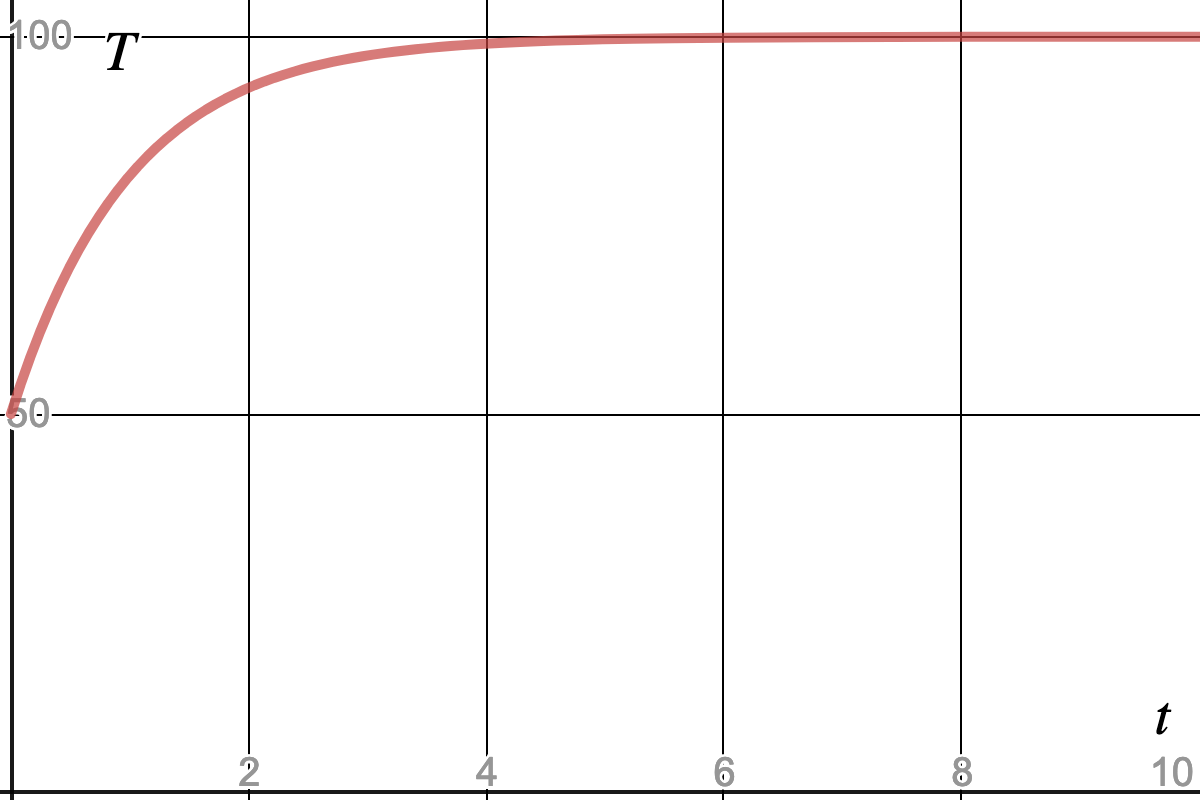
\includegraphics[width=.4\textwidth]{Worksheet_2/desmos-graph(20).png}
\end{figure}
Now we can see the temperature of the object approaches the temperature of the ambient environment as time goes on. This is what we expect!
\end{solution}

\hrule

\begin{problem}
    What happens instead if the initial temperature is equal to the ambient temperature? Does your solution reflect this? Does this make physical sense?
\end{problem}
\begin{solution}
If the initial temperature was equal to the ambient temperature then we don't expect the object to change temperature over time.  One would find that we have the equation
\[
100=T(0)=100-e^{-0-C}=100-e^{-C}
\]
and so $e^{-C}=0$ and thus
\[
T(t)=100,
\]
which is what we expect.
\end{solution}

\hrule

\begin{problem}
    Let $\delta = (T_a-T)$. Show that the equation you found in Problem 1 reduces to
    \[
    \delta' = -k\delta.
    \]
    What is this equation describing physically?
\end{problem}
\begin{solution}
Well, note that $\delta'=(T_a-T)'=-T'$.  Thus we can write
\[
\delta'=-T'=-k(T_a-T)=-k\delta.
\]
This equation is describing how the \emph{difference} in temperature of the object versus the ambient environment will change over time. If you were to solve this, you would find that $\delta\to 0$ as $t\to \infty$.
\end{solution}

\hrule

\begin{center}
    Problems 7-8 are related.
\end{center}
\begin{problem}
    Show that $x=c_1\sin(t)+c_2\cos(t)$ is a general solution to the equation
    \[
        x''+x=0.
    \]
\end{problem}
\begin{solution}
We plug in our guess for $x$ into the left hand side of the equation and we'll check to see that we get zero.  So,
\begin{align*}
    x''+x&=(c_1\sin(t)+c_2\cos(t))''+(c_1\sin(t)+c_2\cos(t))\\
    &= -c_1\sin(t)-c_2\cos(t)+c_1\sin(t)+c_2\cos(t)\\
    &=0.
\end{align*}
Indeed, this $x$ does solve our equation.
\end{solution}

\hrule

\begin{problem}
    Find the particular solution if $x(0)=1$ and $x'(0)=2$. Plot your solution in the $t,x$-plane and in the $x,x'$-plane. 
\end{problem}
\begin{solution}
Now, we use our initial data with our general solution above
\begin{align*}
    1=x(0)=c_1\sin(0)+c_2\cos(0)=c_2
\end{align*}
so $c_2=1$.  Also, we have
\[
0=x'(0)=c_1\cos(0)-\sin(0)=c_1
\]
so $c_1=0$.
\end{solution}

\hrule

\begin{problem}
    Consider the differential equation
    \[
    x'=\frac{x^2+tx+t^2}{tx}.
    \]
    \begin{enumerate}[(a)]
        \item Let $f(x,t)=x^2+tx+t^2$.  Show that $f(\lambda x, \lambda t)=f(x,t)$.
        \item Use the substitution $u=\frac{x}{t}$ in order to make the original equation separable.
        \item Find the general solution to this separable equation in terms of $u$ and $t$. You may use Wolfram Alpha to compute the necessary integral.
        \item Find the solution to the original equation using the substitution $u=\frac{x}{t}$ and your solution from (c).
    \end{enumerate}
\end{problem}
\begin{solution}~
\begin{enumerate}[(a)]
    \item Take
    \begin{align*}
        f(\lambda x, \lambda t) &= \frac{(\lambda x)^2 + (\lambda t)(\lambda x) + (\lambda t)^2}{(\lambda t) (\lambda x)}\\
        &= \frac{\lambda^2 x^2 + \lambda^2 tx + \lambda^2 t^2}{\lambda^2 tx}\\
        &= \frac{x^2+tx+t^2}{tx}.
    \end{align*}
    Indeed we have that $f(\lambda x, \lambda t)=f(x,t)$.
    \item 
\end{enumerate}
\end{solution}


\end{document}
